\section{Zavedení relace}\label{sec:zavedeni_relace}
Relace (jak název napovídá) odpovídá jistému "vztahu". Z reálného života takové příklady známe, např. vztah "matka -- dcera", "stát -- hlavní město státu", apod. Jsou-li např. Jitka a Lenka spolu ve vztahu "matka -- dcera", pak bychom mohli jednoduše psát
\begin{equation*}
    (\text{Jitka}, \text{Lenka}).
\end{equation*}
To~však v řeči matematiky není nic jiného, než uspořádaná dvojice prvků. K tomu se nám bude hodit již zavedený kartézský součin.
\begin{definition}[Relace]\label{def:relace}
    Nechť $X,Y$ jsou libovolné množiny. Pak \emph{relací mezi $X$ a $X$} nazýváme libovolnou podmnožinu $R$ kartézského součinu $X\times Y$, tj. $R\subseteq X \times Y$. Speciálně, pokud $X=Y$, pak mluvíme o \emph{relaci na množině $X$}, tzn. $R\subseteq X^2$.
\end{definition}
Pokud $(x,y)\in R$, pak říkáme, že \emph{prvky $x$ a $y$ jsou v~relaci $R$}, což ekvivalentně zapisujeme jako $xRy$. Jak už jsme si zmínili, tak relace již známe a i v~tomto textu jsme je mnohokrát použili. Např. relace rovnosti "$=$" na $\N$ by obsahovala prvky $(1,1),\,(2,2),\,(3,3),\dots$. Pochopitelně bychom mohli psát "$(2,2)\in\;=$", ale to neděláme; místo toho zkrátka píšeme "$2=2$". Podobně např. relace "$\leq$" na množině $\R$, "$>$", "$\geq$", aj.
\begin{convention}
    Pro značení relací budeme používat velká písmena latinské abecedy $A,B,C,\dots,X,Y,Z$.
\end{convention}
Relace můžeme znázornit více způsoby v~závislosti na jejich typu. Např. máme-li relaci $R=\set{(1,b),\,(1,d),\,(2,d),\,(3,c),\,(4,a)}$ mezi množinami $A=\set{1,2,3,4}$ a $B=\set{1,2,3,4,5}$, pak ji můžeme znázornit způsobem uvedeným na obrázku \ref{fig:relace_mezi_mnozinami}.
\begin{figure}[H]
    \centering
    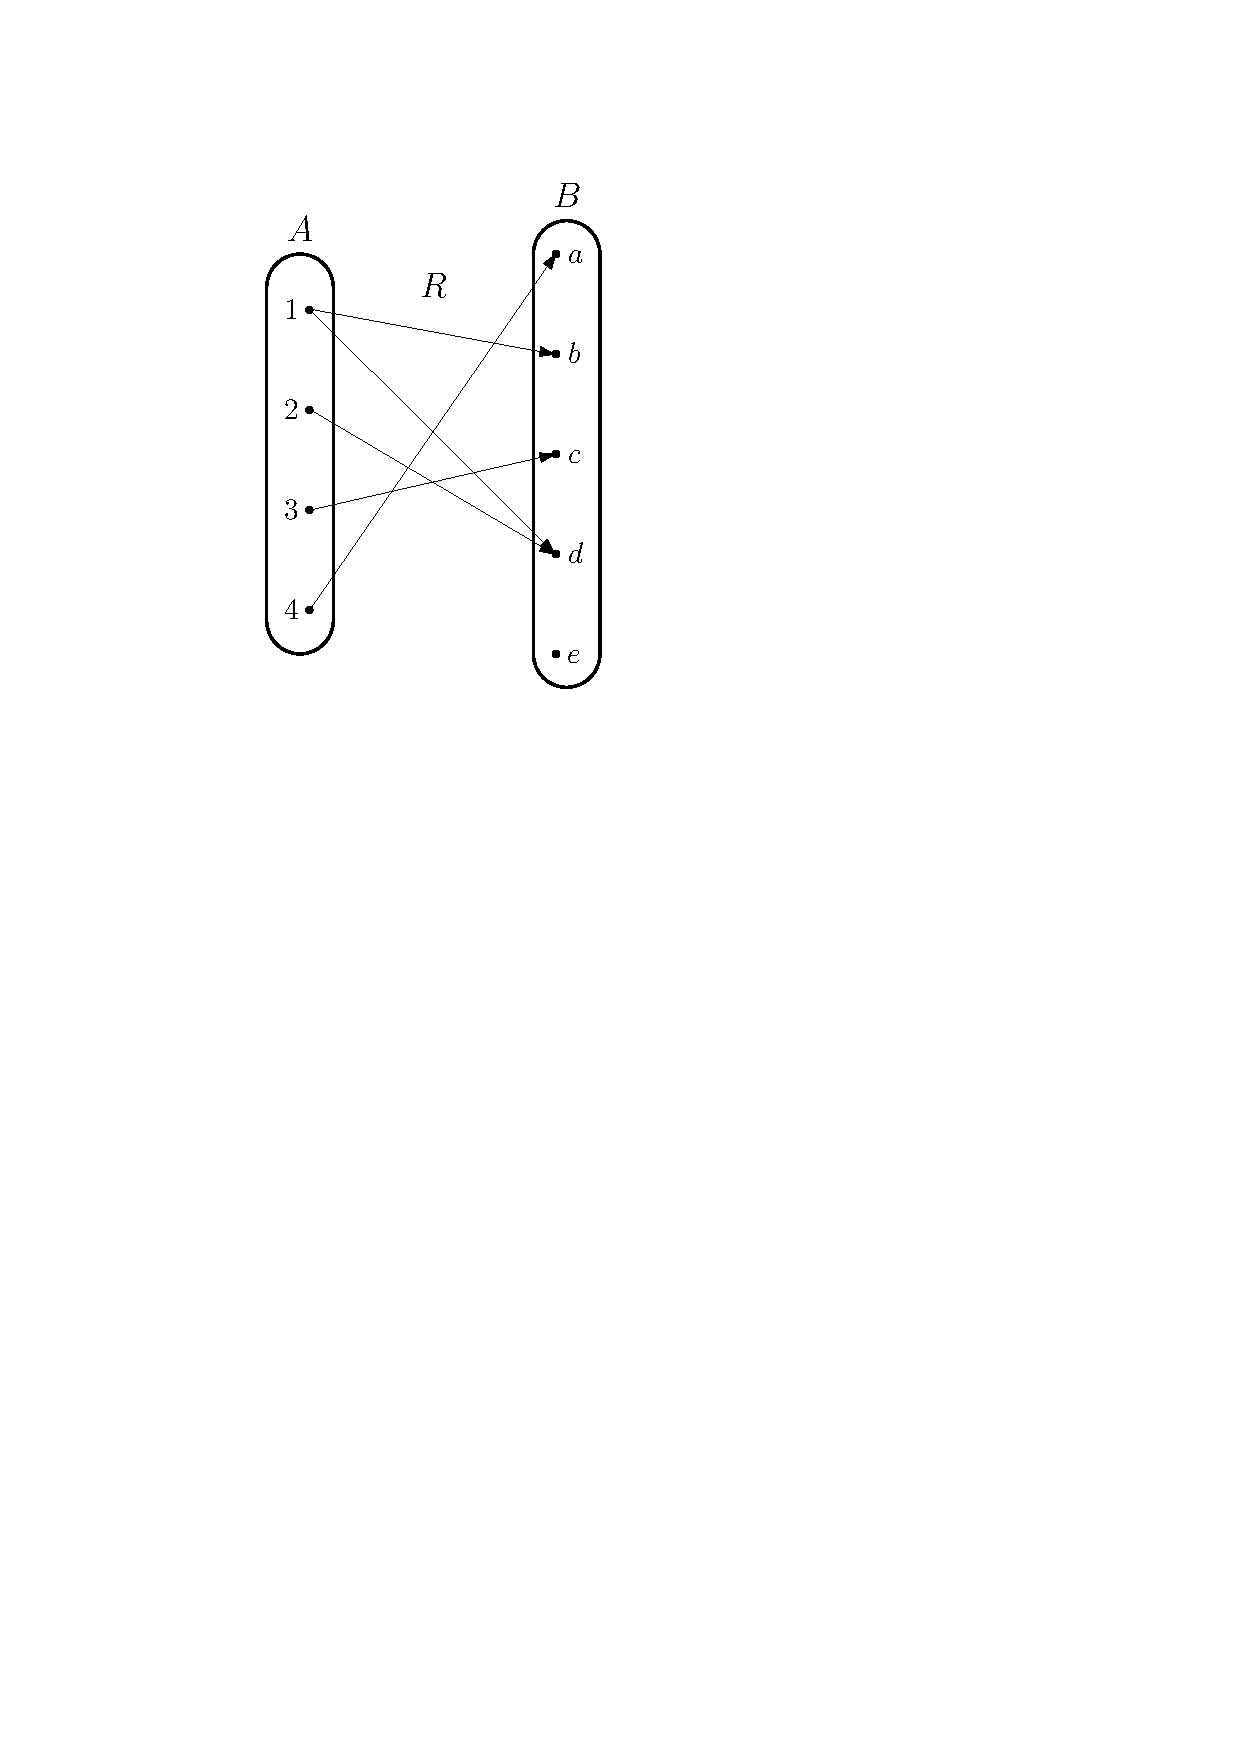
\includegraphics[scale=\normalipe]{ch02_relace_mezi_mnozinami.pdf}
    \caption{Grafické znázornění relace $R$ mezi množinami $A$ a $B$.}
    \label{fig:relace_mezi_mnozinami}
\end{figure}
Avšak pokud máme relaci $S$ \textbf{na množině} $C=\set{x,y,z}$, kupříkladu $S=\set{(x,z),\,(x,y),\,(y,x),\,(z,y),\,(z,z)}$, pak volíme spíše znázornění na obrázku \ref{fig:relace_mezi_mnozinami}.
\begin{figure}[H]
    \centering
    
\includegraphics[scale=\normalipe]{ch02_relace_na_mnozine.pdf}
    \caption{Grafické znázornění relace $S$ na množině $C$.}
    \label{fig:relace_mezi_mnozinami}
\end{figure}
Jako poslední si ještě zmíníme tzv. \emph{skládání relací}.
\begin{definition}[Složení relací]\label{def:skladani_relaci}
    Nechť $X,Y,Z$ jsou libovolné množiny, $R\subseteq X\times Y$ a $S\subseteq Y\times Z$. Relaci $T\subseteq X\times Z$ definujeme následovně:
    \begin{equation*}
        xTz \iff \exists y\in Y : xRy \land ySz.
    \end{equation*}
    Složení relací $R$ a $S$ značíme $S\circ R$, tzn. $T=S\circ R$.
\end{definition}
\begin{example}\label{ex:skladani_relaci}
    Mějme množiny $A=\set{a,b,c}$, $B=\set{x,y,z}$ a $C=\set{i,j,k,l}$. Na nich definujme relace
    \begin{equation*}
        R=\set{(a,z),\,(a,y),\,(c,x)}\subseteq A\times B\quad\text{a}\quad S=\set{(x,k),\,(y,i),\,(y,j),\,(z,j)}\subseteq B\times C.
    \end{equation*}
    Určete $T=S\circ R$.
\end{example}
\begin{solution}
    Postupujme podle definice \ref{def:skladani_relaci} výše. Pro každou z dvojic v $R$ se podíváme, zda existuje nějaká dvojice v $s$ taková, že platí: $t_1Rt_2$ a $t_2St_3$, kde $t_1\in a$ $t_2\in b$ a $t_3\in C$.
    \begin{align*}
        aRj \land zSj &\implies aTj,\\
        aRy \land ySi &\implies aTi,\\
        aRy \land ySj &\implies aTj\;\text{(duplikátní)},\\
        cRx \land xSk &\implies cTk.
    \end{align*}
    Tedy $T=\set{(a,i),\,(a,j),\,(c,k)}$.
\end{solution}
\begin{figure}[H]
    \centering
    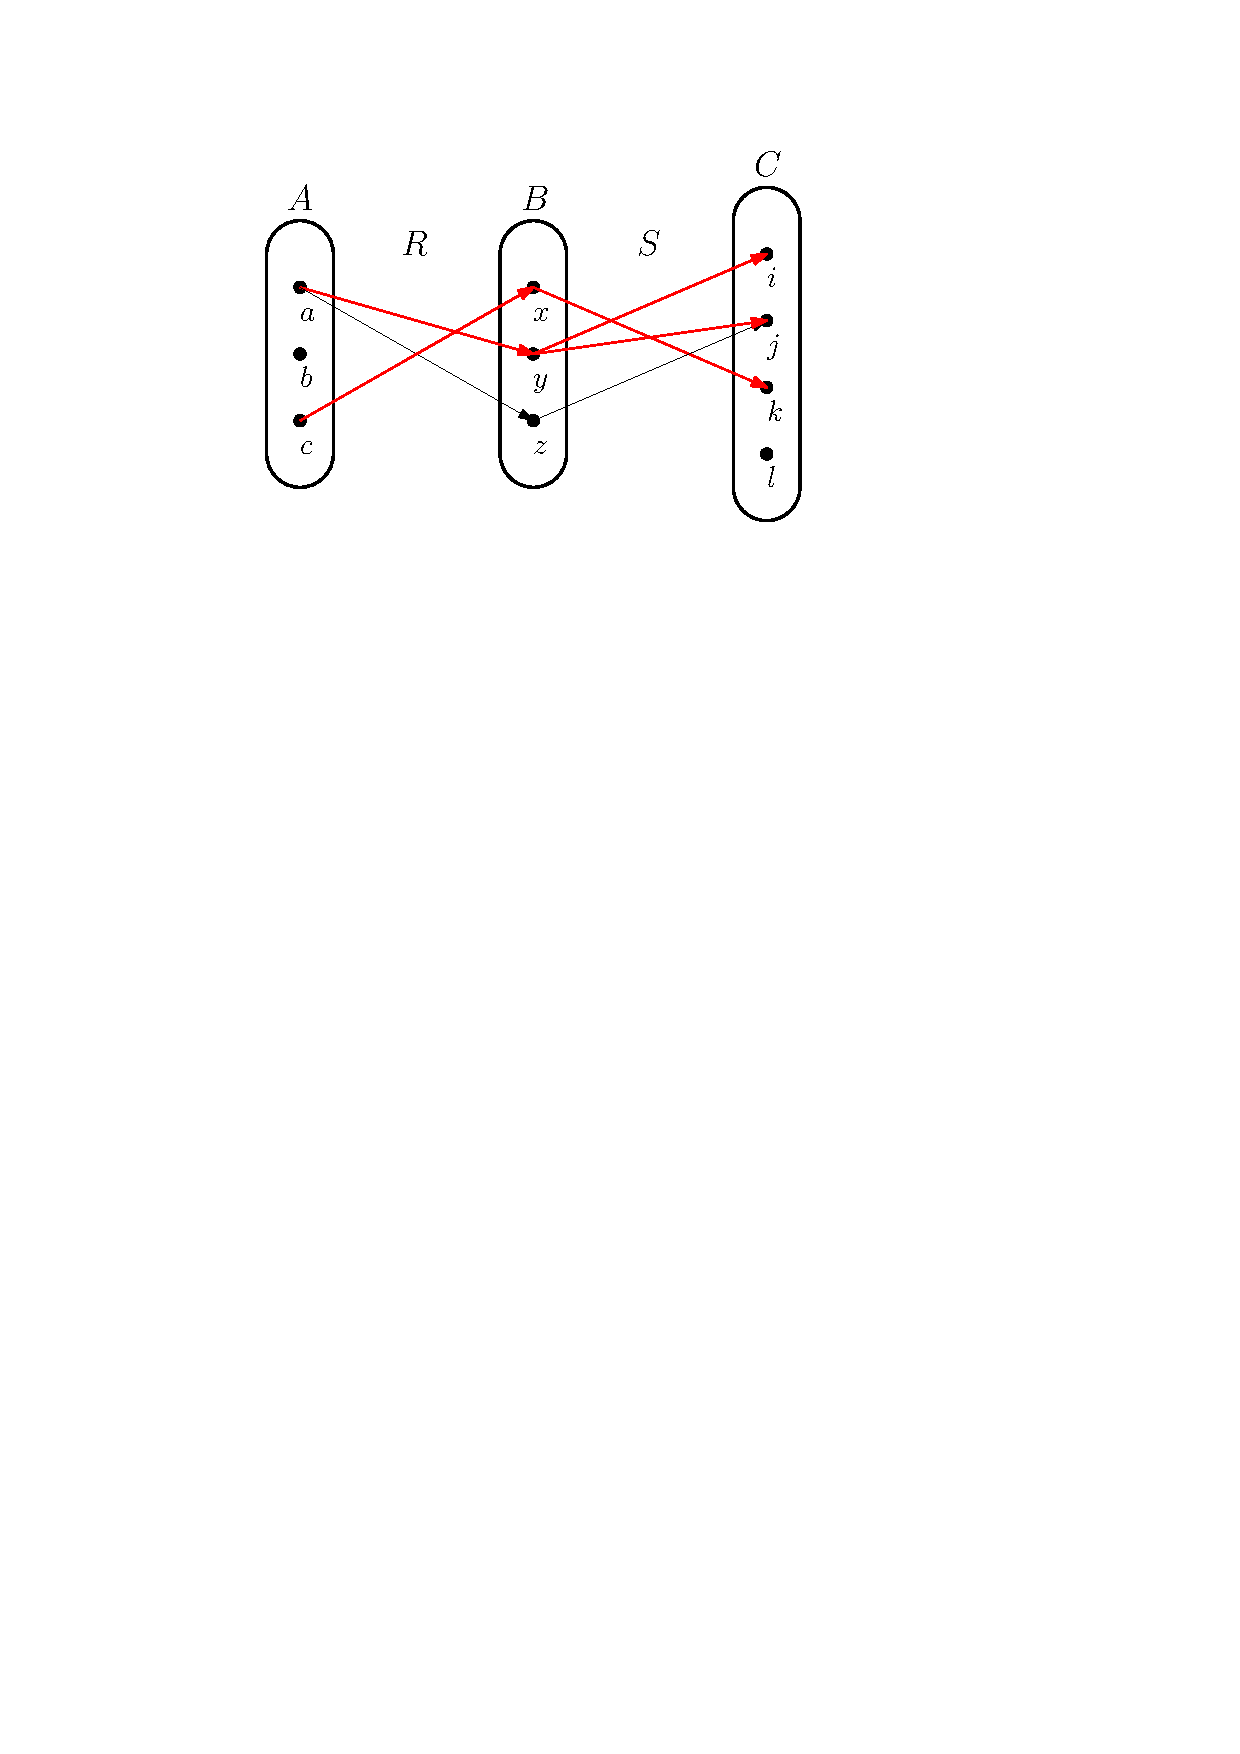
\includegraphics[scale=\normalipe]{ch02_skladani_relaci.pdf}
    \caption{Grafické znázornění relace složení relací $R$ a $S$ z příkladu \ref{ex:skladani_relaci}.}
    \label{fig:relace_mezi_mnozinami}
\end{figure}

Podívejme se ještě na jeden příklad:
\begin{example}\label{ex:skladani_relaci_2}
    Mějme relace $R=\set{(x,x),\,(x,y),\,(y,z)}$ a $S=\set{(x,z),\,(z,y)}$. Určete $T=S\circ R$ a $T^\prime=R\circ S$.
\end{example}
\begin{solution}
    Začneme s $T=S\circ R$.
    \begin{align*}
        xRx \land xSz &\implies xTz\\
        yRz \land zSy &\implies yTy
    \end{align*}
    Tzn. $T=\set{(x,z),\,(y,y)}$. Nyní analogicky pro $T\prime$.
    \begin{align*}
        zSy \land yRz \implies zTz
    \end{align*}
    Tím získáváme $T^\prime=\set{(z,z)}$.
\end{solution}
Z příkladu \ref{ex:skladani_relaci_2} lze vidět, že skládání relací není komutativní a tedy záleží na pořadí.\\
(Sekce inspirována \cite{MatousekNesetril2009}, str. 34--39.)